% =====================================================================
\lecture{1}{משוואות פרידמן, פתרונות, זמנים ומרחקים}{מפגש 1, שעתיים. \ (15' ניוטון, 25' גזירה מ-\en{GR}, 30' פתרונות, 50' זמנים ומרחקים + תרגילים)}
% =====================================================================

\begin{goalbox}
\textbf{מטרות.} (1) לגזור את משוואות פרידמן (ניוטונית, ואז לראות מה \en{GR} מוסיפה). (2) לפתור אותן לרכיב בודד ולחומר${}+\Lambda$. (3) לחשב גיל, זמן מבט-לאחור ושלושת המרחקים $D_M$, $D_A$, $D_L$.
\end{goalbox}

\subsection{התפשטות, מקדם הקנה מידה, הסחה לאדום}
העקרון הקוסמולוגי (הומוגניות ואיזוטרופיות) משאיר דרגת חופש אחת: $a(t)$. מרחק פיזיקלי בין שני גופים נעים: $r=a(t)\,x$, עם $x$ קבוע. גזירה:
\begin{equation}
\dot r=\frac{\dot a}{a}\,r\equiv H(t)\,r \qquad(\text{חוק האבל}).
\end{equation}
אורך הגל נמתח יחד עם המרחב, $\lambda\propto a$, ולכן
\begin{equation}
1+z=\frac{\lambda_{\rm obs}}{\lambda_{\rm em}}=\frac{1}{a(t_{\rm em})} .
\end{equation}
המטריקה (\en{FLRW}), עם $k=0,\pm1$ ו-$S_k(\chi)=\sin\chi,\ \chi,\ \sinh\chi$:
\begin{equation}
ds^2=-c^2dt^2+a^2(t)\left[d\chi^2+S_k^2(\chi)\,d\Omega^2\right].
\end{equation}

\subsection{משוואות פרידמן}
\textbf{גזירה ניוטונית.} כדור ברדיוס $r=ax$ וצפיפות $\rho$. אנרגיה של חלקיק בשפה:
\begin{equation}
\frac12\dot r^2-\frac{GM}{r}=E,\qquad M=\frac{4\pi}{3}\rho r^3
\quad\Longrightarrow\quad
H^2=\frac{8\pi G}{3}\rho-\frac{kc^2}{a^2},
\end{equation}
כאשר $kc^2\equiv-2E/x^2$ קבוע. \emph{האנרגיה הכוללת היא העקמומיות.}

\textbf{הגבול של הגזירה הניוטונית.} היא נותנת את המשוואה הראשונה, אבל לא אומרת מה עושה הלחץ, ומניחה מרחב אוקלידי ואינסופי עם מרכז שרירותי. ב-\en{GR} אין את הבעיות האלה.

\subsection{גזירה מיחסות כללית}
\emph{עובדים ב-$c=1$; בסוף מחזירים $c$. ראשית נגזור את המקרה השטוח ($k=0$) עד הסוף, ואז נוסיף עקמומיות ו-$\Lambda$.}

\textbf{שלב 0: מה צריך.} משוואות איינשטיין, $G_{\mu\nu}\equiv R_{\mu\nu}-\tfrac12g_{\mu\nu}R=8\pi G\,T_{\mu\nu}$, עם
\begin{equation}
\Gamma^\lambda_{\mu\nu}=\tfrac12g^{\lambda\sigma}\big(\partial_\mu g_{\sigma\nu}+\partial_\nu g_{\sigma\mu}-\partial_\sigma g_{\mu\nu}\big),\qquad
R_{\mu\nu}=\partial_\lambda\Gamma^\lambda_{\mu\nu}-\partial_\nu\Gamma^\lambda_{\mu\lambda}+\Gamma^\lambda_{\lambda\sigma}\Gamma^\sigma_{\mu\nu}-\Gamma^\lambda_{\nu\sigma}\Gamma^\sigma_{\mu\lambda}.
\label{eq:ricci-def}
\end{equation}

\textbf{שלב 1: המטריקה.} בקואורדינטות נעות קרטזיות, $ds^2=-dt^2+a^2(t)\,\delta_{ij}dx^idx^j$, כלומר
\begin{equation}
g_{00}=-1,\quad g_{ij}=a^2\delta_{ij},\quad g^{00}=-1,\quad g^{ij}=a^{-2}\delta^{ij}.
\end{equation}
הרכיב היחיד שתלוי במשהו הוא $g_{ij}$, והוא תלוי רק ב-$t$. לכן רק נגזרות $\partial_0g_{ij}=2a\dot a\,\delta_{ij}$ שורדות.

\textbf{שלב 2: סמלי כריסטופל.} מציבים ב-\eqref{eq:ricci-def}. רק שני סוגים אינם אפס:
\begin{equation}
\boxed{\;\Gamma^0_{ij}=a\dot a\,\delta_{ij},\qquad \Gamma^i_{0j}=\Gamma^i_{j0}=\frac{\dot a}{a}\,\delta^i_j=H\delta^i_j\;}
\end{equation}
לדוגמה: $\Gamma^0_{ij}=\tfrac12g^{00}(-\partial_0g_{ij})=\tfrac12\cdot2a\dot a\,\delta_{ij}$. כל השאר ($\Gamma^0_{00}$, $\Gamma^0_{0i}$, $\Gamma^i_{00}$, $\Gamma^i_{jk}$) מתאפסים, כי $g_{00}$ קבוע ו-$g_{ij}$ לא תלוי ב-$x$. \emph{פירוש:} $\Gamma^i_{0j}$ הוא "חיכוך האבל" במשוואת הגאודזה, $\dot p\propto-Hp$, כלומר $p\propto1/a$; לכן אורכי גל נמתחים.

\textbf{שלב 3: טנזור ריצ'י.} הרכיב $00$, איבר אחר איבר ב-\eqref{eq:ricci-def}:
\begin{equation}
R_{00}=\underbrace{\partial_\lambda\Gamma^\lambda_{00}}_{0}-\underbrace{\partial_0\Gamma^\lambda_{0\lambda}}_{\partial_0(3\dot a/a)}+\underbrace{\Gamma^\lambda_{\lambda\sigma}\Gamma^\sigma_{00}}_{0}-\underbrace{\Gamma^\lambda_{0\sigma}\Gamma^\sigma_{0\lambda}}_{\Gamma^i_{0j}\Gamma^j_{0i}=3H^2}
=-3\Big(\frac{\ddot a}{a}-\frac{\dot a^2}{a^2}\Big)-3\frac{\dot a^2}{a^2}
=-3\frac{\ddot a}{a}.
\end{equation}
הרכיבים $ij$:
\begin{equation}
R_{ij}=\underbrace{\partial_0\Gamma^0_{ij}}_{(\dot a^2+a\ddot a)\delta_{ij}}-\underbrace{\partial_j\Gamma^\lambda_{i\lambda}}_{0}+\underbrace{\Gamma^\lambda_{\lambda0}\Gamma^0_{ij}}_{3H\cdot a\dot a\,\delta_{ij}}-\underbrace{\big(\Gamma^0_{jk}\Gamma^k_{i0}+\Gamma^k_{j0}\Gamma^0_{ik}\big)}_{2\dot a^2\delta_{ij}}
=\big(a\ddot a+2\dot a^2\big)\delta_{ij}.
\end{equation}
$R_{0i}=0$ מאיזוטרופיות: אין כיוון מועדף שאליו וקטור יכול להצביע.

\textbf{שלב 4: סקלר ריצ'י וטנזור איינשטיין.}
\begin{equation}
R=g^{00}R_{00}+g^{ij}R_{ij}=3\frac{\ddot a}{a}+\frac{3(a\ddot a+2\dot a^2)}{a^2}=6\Big(\frac{\ddot a}{a}+\frac{\dot a^2}{a^2}\Big),
\end{equation}
\begin{equation}
\boxed{\;G_{00}=R_{00}+\tfrac12R=3\frac{\dot a^2}{a^2},\qquad
G_{ij}=R_{ij}-\tfrac12a^2\delta_{ij}R=-\big(2a\ddot a+\dot a^2\big)\delta_{ij}\;}
\end{equation}
שימו לב: ב-$G_{00}$ \emph{אין} $\ddot a$. זו משוואת אילוץ (כמו חוק גאוס באלקטרומגנטיות), לא משוואת תנועה.

\textbf{שלב 5: המקור.} נוזל מושלם במנוחה בקואורדינטות הנעות, $u^\mu=(1,0,0,0)$, $u_\mu=(-1,0,0,0)$:
\begin{equation}
T_{\mu\nu}=(\rho+p)u_\mu u_\nu+p\,g_{\mu\nu}\quad\Longrightarrow\quad T_{00}=\rho,\qquad T_{ij}=p\,a^2\delta_{ij}.
\end{equation}
זו הצורה היחידה שמתאימה לסימטריה: הומוגניות דורשת $\rho(t)$, $p(t)$, ואיזוטרופיות דורשת $T_{0i}=0$ ו-$T_{ij}\propto\delta_{ij}$.

\textbf{שלב 6: שתי המשוואות.}
\begin{align}
00:\qquad &3\frac{\dot a^2}{a^2}=8\pi G\rho &&\Longrightarrow\quad H^2=\frac{8\pi G}{3}\rho ,\\
ij:\qquad &-\big(2a\ddot a+\dot a^2\big)=8\pi G\,p\,a^2 &&\Longrightarrow\quad 2\frac{\ddot a}{a}+H^2=-8\pi Gp .
\end{align}
מציבים את $H^2$ מהראשונה בשנייה: $2\ddot a/a=-8\pi G(p+\rho/3)$, כלומר
\begin{equation}
\frac{\ddot a}{a}=-\frac{4\pi G}{3}\big(\rho+3p\big).
\end{equation}

\textbf{שלב 7: שימור, בחינם.} זהות ביאנקי $\nabla^\mu G_{\mu\nu}\equiv0$ מחייבת $\nabla^\mu T_{\mu\nu}=0$. הרכיב $\nu=0$:
\begin{equation}
\nabla_\mu T^{\mu0}=\partial_0T^{00}+\Gamma^\mu_{\mu0}T^{00}+\Gamma^0_{ij}T^{ij}
=\dot\rho+3H\rho+a\dot a\,\delta_{ij}\,\frac{p}{a^2}\delta^{ij}
=\dot\rho+3H(\rho+p)=0 .
\end{equation}
אותה תוצאה מתקבלת אם גוזרים את משוואת $00$ בזמן ומציבים את משוואת $ij$. לכן רק \emph{שתיים} משלוש המשוואות בלתי תלויות. בפועל עובדים עם פרידמן הראשונה ומשוואת השימור.

\textbf{שלב 8: עקמומיות ו-$\Lambda$.}
\begin{itemize}
\item \textbf{$k\neq0$.} עם $g_{ij}=a^2\gamma_{ij}$, כאשר $\gamma_{ij}$ מטריקה של מרחב בעל עקמומיות קבועה, למרחב הזה יש ריצ'י משלו: ${}^{(3)}\!R_{ij}=2k\gamma_{ij}$. התוצאה: $G_{00}=3\big(H^2+k/a^2\big)$ ו-$G_{ij}=-\big(2a\ddot a+\dot a^2+k\big)\gamma_{ij}$. המשוואה הראשונה מקבלת $-k/a^2$; משוואת התאוצה לא משתנה ($k$ מתבטל בהפרש).
\item \textbf{$\Lambda$.} $G_{\mu\nu}+\Lambda g_{\mu\nu}=8\pi GT_{\mu\nu}$. העברה לאגף ימין מראה ש-$\Lambda$ הוא נוזל עם $\rho_\Lambda=\Lambda/8\pi G$ ו-$p_\Lambda=-\rho_\Lambda$. שימו לב ש-$\rho_\Lambda+3p_\Lambda=-2\rho_\Lambda<0$: כבידה דוחה.
\end{itemize}
מחזירים $c$ ($\rho\to\rho c^2$ בצפיפות אנרגיה, $k\to kc^2$, $\Lambda\to\Lambda c^2$) ומקבלים:
\begin{equation}
\boxed{\;H^2=\frac{8\pi G}{3}\rho-\frac{kc^2}{a^2}+\frac{\Lambda c^2}{3},\qquad
\frac{\ddot a}{a}=-\frac{4\pi G}{3}\Big(\rho+\frac{3p}{c^2}\Big)+\frac{\Lambda c^2}{3}\;}
\label{eq:friedmann}
\end{equation}

\begin{keybox}
\textbf{תסריט ללוח (כ-25 דקות).} מטריקה $\to$ שני סוגי $\Gamma$ $\to$ $R_{00}$ ו-$R_{ij}$ (לעשות לפחות את $R_{00}$ איבר אחר איבר) $\to$ $R$ $\to$ $G_{00}$, $G_{ij}$ $\to$ $T_{\mu\nu}$ $\to$ שתי משוואות $\to$ ביאנקי נותן שימור. \emph{נקודות לעצור עליהן:} (1) $G_{00}$ בלי $\ddot a$ = אילוץ; (2) $\rho+3p$ במשוואת התאוצה; (3) $k$ נכנס דרך העקמומיות של המרחב התלת-ממדי, לא דרך $a$.
\end{keybox}

ההבדל המהותי: \textbf{הלחץ כובד}. זה מה שניוטון לא יכול לתת, ובזכותו $p<-\rho c^2/3$ מאיץ.
משוואת השימור (שלב 7; או בתרמודינמיקה, $dE=-p\,dV$) נותנת את התלות של כל רכיב ב-$a$:
\begin{equation}
\dot\rho+3H\Big(\rho+\frac{p}{c^2}\Big)=0
\quad\xrightarrow{\;p=w\rho c^2\;}\quad
\rho\propto a^{-3(1+w)}:\qquad
\begin{cases}
\text{חומר } (w=0): & \rho\propto a^{-3}\\
\text{קרינה } (w=\tfrac13): & \rho\propto a^{-4}\\
\Lambda\ (w=-1): & \rho=\text{const}
\end{cases}
\end{equation}

\textbf{פרמטרי צפיפות.} $\rho_c=3H^2/8\pi G$, $\Omega_i=\rho_i/\rho_c$, $\Omega_k=-kc^2/(a_0H_0)^2$. היום $\sum_i\Omega_{i}+\Omega_k=1$, ומשוואת פרידמן הופכת ל:
\begin{equation}
\boxed{\;E^2(z)\equiv\frac{H^2}{H_0^2}=\Omega_r(1+z)^4+\Omega_m(1+z)^3+\Omega_k(1+z)^2+\Omega_\Lambda\;}
\label{eq:Ez}
\end{equation}
ופרמטר התאוטה $q\equiv-\ddot a a/\dot a^2$ נותן היום $q_0=\tfrac12\Omega_m+\Omega_r-\Omega_\Lambda$.

\subsection{פתרונות}
\begin{keybox}
\textbf{רכיב בודד, $k=0$.} $\dot a^2\propto a^{-(1+3w)}$ נותן
\begin{equation}
a\propto t^{2/[3(1+w)]}:\qquad a\propto t^{1/2}\ (\text{קרינה}),\quad a\propto t^{2/3}\ (\text{חומר, \en{EdS}}),\quad a\propto e^{H_\Lambda t}\ (\Lambda).
\end{equation}
ב-\en{EdS}: $H=2/(3t)$, ולכן $t_0=\frac23H_0^{-1}=9.3\,\Gyr$ עבור $h=0.7$ --- צעיר מהכוכבים הזקנים ביותר ($\gtrsim12\,\Gyr$). זו הייתה רמז מוקדם ל-$\Lambda$.
\end{keybox}

\textbf{חומר${}+\Lambda$ ($k=0$), פתרון סגור.} עם $x=a^{3/2}$ המשוואה הופכת למשוואה לינארית ופתרונה
\begin{equation}
a(t)=\Big(\frac{\Omega_m}{\Omega_\Lambda}\Big)^{1/3}\sinh^{2/3}\!\Big(\tfrac32\sqrt{\Omega_\Lambda}\,H_0t\Big),
\qquad
t_0=\frac{2}{3H_0\sqrt{\Omega_\Lambda}}\,\mathrm{arsinh}\sqrt{\frac{\Omega_\Lambda}{\Omega_m}} .
\end{equation}
\textbf{מעברים.} $\rho_r=\rho_m$ ב-$1+z_{\rm eq}=\Omega_m/\Omega_r\approx3400$; $\rho_m=\rho_\Lambda$ ב-$z\approx0.33$; התאוצה מתחילה ($\ddot a=0$) ב-$1+z_{\rm acc}=(2\Omega_\Lambda/\Omega_m)^{1/3}$, כלומר $z_{\rm acc}\approx0.67$.

\textbf{עקמומיות.} ביקום של חומר בלבד: $k=+1$ קורס, $k=-1$ מתפשט לנצח ($a\propto t$ בגבול), $k=0$ על הגבול. עם $\Lambda$ הגורל נקבע על ידי $\Lambda$, לא על ידי $k$. העקמומיות דועכת לאט יותר מחומר וקרינה ($a^{-2}$), ולכן היא שולטת בעתיד אם $\Lambda=0$; זו "בעיית השטיחות" של הרצאה 6.

\begin{figure}[htbp]\centering
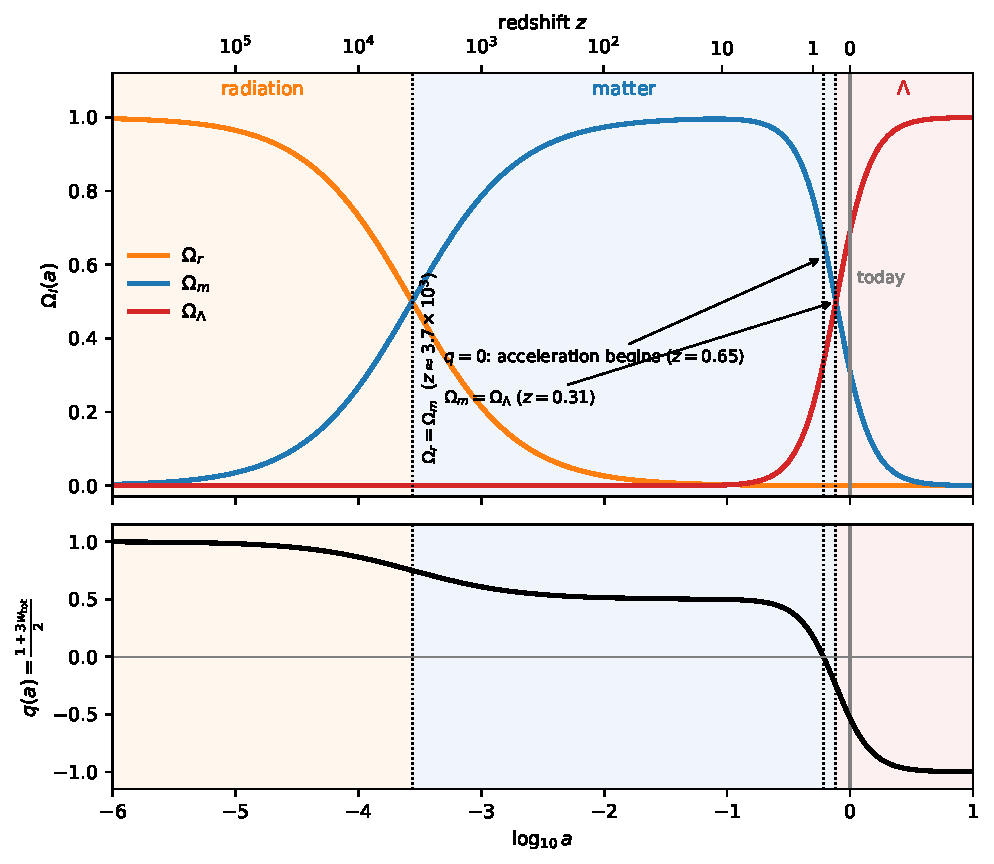
\includegraphics[width=0.75\textwidth]{figs/fig_omega_z.pdf}
\caption{\small $\Omega_i(z)$: עידן קרינה, עידן חומר ועידן $\Lambda$. המעברים ב-$z_{\rm eq}\approx3400$ וב-$z\approx0.3$.}
\end{figure}

\subsection{זמנים}
מ-$dt=da/(aH)$:
\begin{equation}
t(z)=\int_z^\infty\frac{dz'}{(1+z')H(z')},\qquad
t_{\rm lb}(z)=\int_0^z\frac{dz'}{(1+z')H(z')} .
\end{equation}
עבור $\Omega_m=0.3$, $h=0.7$: $t_0=13.5\,\Gyr$, ואור מ-$z=1$ יצא לפני $7.7\,\Gyr$. עם ערכי \en{Planck}: $t_0=13.8\,\Gyr$.

\textbf{אופק החלקיק} --- המרחק הנע הגדול ביותר שאור עבר מאז $t=0$: $\chi_{\rm p}=\int_0^{t}c\,dt'/a=\int_z^\infty c\,dz'/H$. ב-\en{EdS} $\chi_{\rm p}=2c/(a H)$, כלומר סופי. בגלל זה יש "בעיית אופק" (הרצאה 6).

\subsection{מרחקים}
כל המרחקים נבנים מהמרחק הנע לאורך קו הראייה (אור נע על $ds=0$, $c\,dt=a\,d\chi$):
\begin{keybox}
\begin{align}
D_C(z)&=\frac{c}{H_0}\int_0^z\frac{dz'}{E(z')},\\
D_M&=\frac{c}{H_0\sqrt{|\Omega_k|}}\,S_k\!\Big(\sqrt{|\Omega_k|}\,\frac{H_0D_C}{c}\Big)\ \ (=D_C\ \text{אם}\ k=0),\\
D_A&=\frac{D_M}{1+z}\quad(\text{גודל זוויתי: } \theta=\ell/D_A),\qquad
D_L=(1+z)\,D_M\quad(\text{שטף: } F=L/4\pi D_L^2).
\end{align}
יחס הדואליות $D_L=(1+z)^2D_A$ נכון בכל מטריקה שבה פוטונים נשמרים. שני גורמי $(1+z)$ ב-$D_L$: האנרגיה של כל פוטון יורדת, וקצב ההגעה שלהם יורד.
\end{keybox}
\textbf{גבול $z\ll1$:} $D\simeq cz/H_0\,[1+\tfrac12(1-q_0)z]$ ($D_L$). כלומר בסדר ראשון מודדים $H_0$, ובסדר שני את $q_0$, את התאוצה.

\textbf{תכונה מפתיעה של $D_A$:} הוא אינו מונוטוני. מעבר ל-$z\sim1.6$ (ב-$\LCDM$) גלקסיה נראית \emph{גדולה} יותר ככל שהיא רחוקה יותר, כי האור יצא כשהיקום היה קטן.

\begin{figure}[htbp]\centering
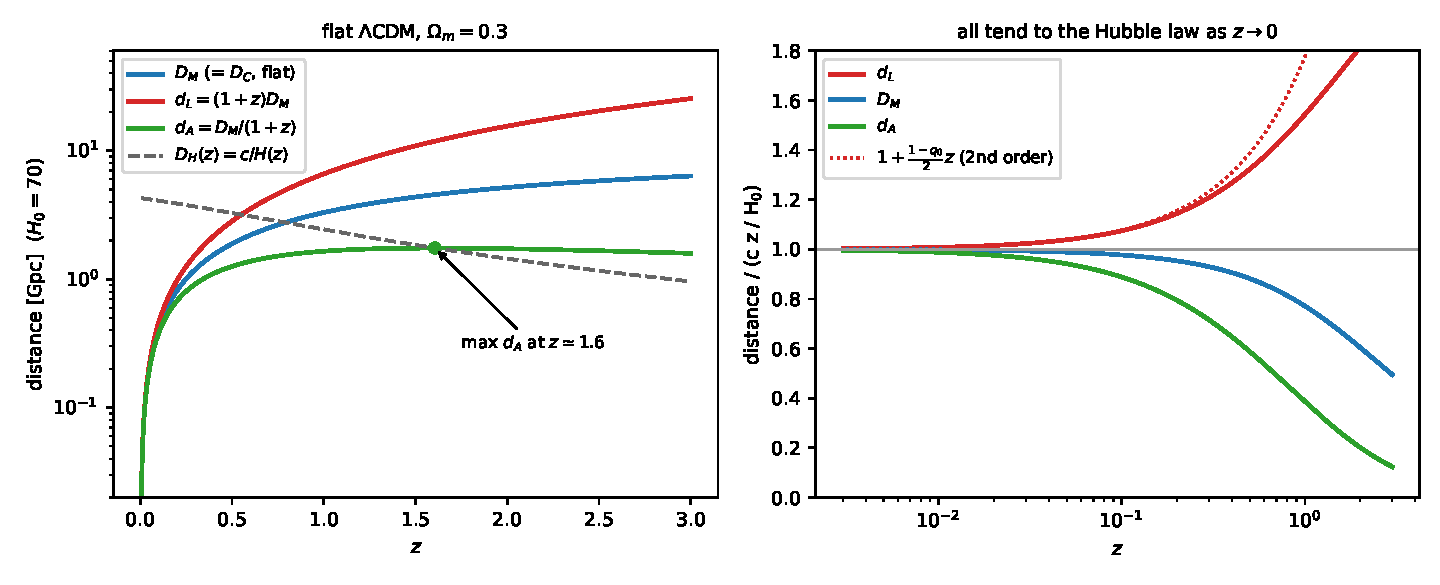
\includegraphics[width=0.95\textwidth]{figs/fig_dist_four.pdf}
\caption{\small ארבעת המרחקים ב-$\LCDM$ שטוח. $D_L$ עולה מהר, $D_A$ מגיע למקסימום ויורד, ו-$D_M$ שואף לאופק.}
\end{figure}

\begin{warnbox}
\textbf{מלכודות נפוצות.} (1) $v=cz$ נכון רק כש-$z\ll1$; ב-$z>1$ גלקסיות "בורחות" מהר מ-$c$ בלי סתירה ליחסות. (2) "מרחק" בלי לציין איזה --- חסר משמעות. (3) $D_M$ ולא $D_C$ הוא שנכנס ל-$D_A$ ול-$D_L$ כש-$k\neq0$.
\end{warnbox}

% ---------------------------------------------------------------------
\subsection*{תרגילים}
\begin{exercise}{גיל ותאוצה}
(א) חשבו את $t_0$ ב-\en{EdS} וב-$\LCDM$ שטוח עם $\Omega_m=0.3$, עבור $h=0.7$.
(ב) מצאו את ההסחה $z_{\rm acc}$ שבה $\ddot a=0$, ואת ההסחה שבה $\rho_m=\rho_\Lambda$. למה הן שונות?
(ג) מה $q_0$? מה הסימן שלו אומר?
\end{exercise}
\begin{solbox}
\textbf{פתרון.}
\textbf{(א)} זמן האבל: $1/H_0=977.8/h\,\Gyr=13.97\,\Gyr$ עבור $h=0.7$ (כי $1\,\Mpc/(1\,\kms)=977.8\,\Gyr$).
\begin{itemize}
\item \en{EdS}: $a\propto t^{2/3}\Rightarrow H=\frac{2}{3t}\Rightarrow t_0=\frac{2}{3H_0}=9.3\,\Gyr$.
\item $\LCDM$: מפתרון $\sinh$, בדרישה $a(t_0)=1$: $\sinh\!\big(\tfrac32\sqrt{\Omega_\Lambda}H_0t_0\big)=\sqrt{\Omega_\Lambda/\Omega_m}=1.528$. מכאן $\tfrac32\sqrt{0.7}\,H_0t_0=\mathrm{arsinh}(1.528)=1.210$, כלומר $H_0t_0=0.964$ ו-$t_0=13.5\,\Gyr$.
\end{itemize}
בדיקה: $t_0=H_0^{-1}\int_0^1\frac{da}{a\sqrt{\Omega_m a^{-3}+\Omega_\Lambda}}$ נותן אותו מספר נומרית. ה-$\Lambda$ "מאריך" את הגיל, כי בעבר ההתפשטות הייתה איטית יותר.

\textbf{(ב)} משוואת התאוצה עם $p_m=0$, $p_\Lambda=-\rho_\Lambda$:
\[
\frac{\ddot a}{a}=-\frac{4\pi G}{3}\big(\rho_m-2\rho_\Lambda\big)=0\ \Longrightarrow\ \rho_m=2\rho_\Lambda
\ \Longrightarrow\ \Omega_m(1+z)^3=2\Omega_\Lambda,
\]
\[
1+z_{\rm acc}=\Big(\frac{2\Omega_\Lambda}{\Omega_m}\Big)^{1/3}=\Big(\frac{1.4}{0.3}\Big)^{1/3}=1.67\ \Rightarrow\ z_{\rm acc}=0.67 .
\]
$\rho_m=\rho_\Lambda$: $(1+z)^3=\Omega_\Lambda/\Omega_m=2.33\Rightarrow z=0.33$. ההבדל: בתאוצה קובע $\rho+3p$, ולא $\rho$. ל-$\Lambda$ יש $\rho+3p=-2\rho$, ולכן "משקלו" כפול, והתאוצה מתחילה \emph{לפני} ש-$\Lambda$ שולט בצפיפות.

\textbf{(ג)} $q_0=\tfrac12\Omega_m-\Omega_\Lambda=0.15-0.70=-0.55$. $q_0<0\iff\ddot a>0$: היקום מאיץ היום. ב-\en{EdS} $q_0=+\tfrac12$ (מאט).
\end{solbox}

\begin{exercise}{המקסימום של $D_A$}
ב-\en{EdS}: (א) הראו ש-$D_C=\frac{2c}{H_0}\big(1-(1+z)^{-1/2}\big)$. (ב) מצאו את $z$ שבו $D_A$ מקסימלי ואת ערכו. (ג) גלקסיה בקוטר $30\,\kpc$: מה גודלה הזוויתי המינימלי (עבור $h=0.7$)?
\end{exercise}
\begin{solbox}
\textbf{פתרון.}
\textbf{(א)} ב-\en{EdS} $E(z)=(1+z)^{3/2}$:
\[
D_C=\frac{c}{H_0}\int_0^z(1+z')^{-3/2}dz'=\frac{c}{H_0}\Big[-2(1+z')^{-1/2}\Big]_0^z=\frac{2c}{H_0}\Big(1-\frac{1}{\sqrt{1+z}}\Big).
\]
ב-$z\to\infty$: $D_C\to2c/H_0$ --- זה אופק החלקיק היום.

\textbf{(ב)} $D_A=D_C/(1+z)$ (שטוח). נציב $u\equiv(1+z)^{-1/2}$, כך ש-$1/(1+z)=u^2$:
\[
D_A=\frac{2c}{H_0}\,u^2(1-u),\qquad \frac{d}{du}\big(u^2-u^3\big)=2u-3u^2=0\ \Rightarrow\ u=\frac23 .
\]
מכאן $1+z=9/4$, כלומר $z=1.25$, ו-
\[
D_A^{\max}=\frac{2c}{H_0}\cdot\frac49\cdot\frac13=\frac{8}{27}\frac{c}{H_0}=0.296\times4283\,\Mpc=1270\,\Mpc .
\]
\textbf{(ג)} $\theta=\ell/D_A\ge\ell/D_A^{\max}$:
\[
\theta_{\min}=\frac{30\,\kpc}{1270\,\Mpc}=2.4\times10^{-5}\ \text{רד'}=4.9'' .
\]
\emph{פירוש:} מעבר ל-$z=1.25$ גלקסיה נראית \emph{גדולה} יותר ככל שהיא רחוקה יותר. האור יצא כשהיקום היה קטן והגלקסיה הייתה קרובה אלינו. ב-$\LCDM$ המקסימום זז ל-$z\approx1.6$.
\end{solbox}

\begin{exercise}{מתי הקרינה שלטה?}
(א) מ-$\Omega_\gamma h^2=2.47\times10^{-5}$ ו-$\Omega_rh^2\simeq4.2\times10^{-5}$ (עם נייטרינו) ו-$\Omega_mh^2=0.143$, חשבו את $z_{\rm eq}$. (ב) מה הטמפרטורה של הקרינה אז ($T=T_0(1+z)$)? (ג) מצאו $a(t)$ ביקום של קרינה${}+$חומר בלבד בעזרת זמן קונפורמי $\eta$ ($dt=a\,d\eta$). רמז: $a(\eta)=a_{\rm eq}\big[(\eta/\eta_*)^2+2\eta/\eta_*\big]$.
\end{exercise}
\begin{solbox}
\textbf{פתרון.}
\textbf{(א)} $\rho_r\propto a^{-4}$ ו-$\rho_m\propto a^{-3}$, ולכן $\rho_r/\rho_m=(\Omega_r/\Omega_m)(1+z)$. שוויון:
\[
1+z_{\rm eq}=\frac{\Omega_m}{\Omega_r}=\frac{\Omega_mh^2}{\Omega_rh^2}=\frac{0.143}{4.2\times10^{-5}}\approx3400 .
\]
(היחס ב-$h^2$ מבטל את התלות ב-$H_0$. בלי נייטרינו היינו מקבלים 5800 --- הנייטרינו חשובים.)

\textbf{(ב)} $T=T_0(1+z)=2.7255\times3400\approx9300\,\mathrm K$, כלומר $k_BT\approx0.80\,\mathrm{eV}$.

\textbf{(ג)} עם $dt=a\,d\eta$ נסמן $a'=da/d\eta=a^2H$. משוואת פרידמן ($k=\Lambda=0$):
\[
a'^2=a^4H^2=H_0^2\big(\Omega_r+\Omega_m a\big).
\]
גוזרים לפי $\eta$: $2a'a''=H_0^2\Omega_m a'$, כלומר $a''=\tfrac12H_0^2\Omega_m=$ קבוע. אינטגרציה עם $a(0)=0$ ו-$a'(0)=H_0\sqrt{\Omega_r}$:
\[
a(\eta)=\frac{\Omega_mH_0^2}{4}\eta^2+\sqrt{\Omega_r}\,H_0\eta
=a_{\rm eq}\Big[\Big(\frac{\eta}{\eta_*}\Big)^2+2\frac{\eta}{\eta_*}\Big],\qquad
a_{\rm eq}=\frac{\Omega_r}{\Omega_m},\ \ \eta_*=\frac{2\sqrt{\Omega_r}}{\Omega_mH_0}.
\]
בדיקת גבולות: $\eta\ll\eta_*$: $a\propto\eta$, ו-$t=\int a\,d\eta\propto\eta^2$, ולכן $a\propto t^{1/2}$ (קרינה). $\eta\gg\eta_*$: $a\propto\eta^2$, $t\propto\eta^3$, ולכן $a\propto t^{2/3}$ (חומר). השוויון $a=a_{\rm eq}$ ב-$\eta/\eta_*=\sqrt2-1$.
\end{solbox}
